%-*- coding: utf-8 -*-
\section{早上がりを目指す貪欲な手法}
早く上がることに対する指標として,早上がりを目指す貪欲な手法がある~\cite{zentu}.役を考えず上がりに必要な組み合わせに貪欲に近づけるように牌を切り,手牌の向聴数を効率良く下げていく.手法の概要としては,手牌の向聴数が変わらない牌の中から有効牌の残り枚数が最も多くなるような牌を捨てるというものである.この手法をAlgorithm~\ref{soboku}に示す.手牌の$s$番目の牌$T_s$を捨てることになる.牌の向聴数はハッシュテーブルを用いて計算している~\cite{syanten}.数牌の組み合わせにおける順子,刻子の数と順子候補,刻子候補の数をハッシュテーブルに持っておき,その値を用いて向聴数を求めている.

\begin{algorithm}[t]
\caption{早上がりを目指す貪欲な手法}
\label{soboku}
	\KwIn{手牌$T$}
	有効牌の枚数を格納する要素数14の配列$Y$の各要素を0にする\;
	\For{$i=1$ \KwTo $14$}{
		手牌から$i$番目の牌を抜く\;
		\If{手牌の向聴数が変わらない}{
			$Y_i \leftarrow$手牌の有効牌の残り枚数\;  
		}
 }
 $s \leftarrow \argmax_{1 \le i \le 14} Y_i$\;
 \Return $T_s$\;
\end{algorithm}

\section{モンテカルロ法}
モンテカルロ法~\cite{montecarlo}は,ゲームを最後まで行うシミュレーションを繰り返し,行動にシミュレーションの結果による報酬を与える.このシミュレーションを\textbf{プレイアウト}と呼ぶ.報酬の合計を価値と呼び,最も価値が高い行動を選択する.プレイアウト時の不確定情報や,プレイヤの行動はランダムに決める.一般的なモンテカルロ法をAlgorithm~\ref{monte}に示す.$N$はプレイアウト回数である.また,一人麻雀におけるモンテカルロ法をAlgorithm~\ref{majangmonte}に示す.しかし,モンテカルロ法を一人麻雀に適用すると,プレイアウト中の行動選択をランダムに行うため,ほとんどのプレイアウトで報酬を得られない.そのため,行動の良さをうまく評価できず,良い行動選択を行えない.モンテカルロ法は一人麻雀において効率の悪い手法である.

\begin{algorithm}[t]
\caption{モンテカルロ法}
\label{monte}
	\KwIn{可能な行動$B$}
	価値を格納する配列$V$の各要素を0にする\;
	\For{$i=1$ \KwTo 可能な行動の個数}{
		盤面において不確定な情報を仮定する\;
		\For{$j=1$ \KwTo $N$}{
			$i$番目の行動を行う\;
			\While{ゲームが終了していない}{
				行動をランダムに決定し,ゲームを進める\;
			}
			$V_i \leftarrow V_i +$ゲームの結果による報酬\; 
		}
	}
	$s \leftarrow \argmax_i V_i$\;
	\Return $B_s$\;
\end{algorithm}

\begin{algorithm}[t]
\caption{一人麻雀におけるモンテカルロ法}
\label{majangmonte}
	\KwIn{手牌$T$}
	価値を格納する要素数14の配列$V$の各要素を0にする\;
	\For{$i=1$ \KwTo $14$}{
		\For{$j=1$ \KwTo $N$}{
			$i$番目の牌を捨てる\;
			\For{$k=1$ \KwTo 残り巡目数}{
				ランダムに1枚の牌を手牌に加える\;
				\If{手牌が上がり条件を満たしている}{
					$V_i \leftarrow V_i +$報酬(上がり点)\; 
					\textbf{break}\;
				}
				ランダムに1枚の牌を手牌から捨てる\;
			}
		}
	}
	$s \leftarrow \argmax_{1 \le i \le 14} V_i$\;
	\Return $T_s$\;
\end{algorithm}
\clearpage

\section{小松らの手法}
小松らの手法~\cite{komatu}はモンテカルロ法を基にしており,一人麻雀に効率の良いプレイアウトを行っている.以下にプレイアウトの手順を示す.
\begin{enumerate}
\item 将来得られる牌を,残り巡目数だけランダムに仮定する.
\item これらの牌と手牌で上がり点が最大となると組み合わせを求める.
\item 求めた組み合わせに含まれない手牌の牌に,上がり点を報酬として与える.
\end{enumerate}
このプレイアウトについて例を用いて説明する.残り巡目が8巡のときの手牌と将来得られる牌を仮定した例を図~\ref{tehaifuture}に示す.このとき,手牌と仮定した牌で上がり点が最大となる組み合わせは図~\ref{maxcombination}のようになる.この組み合わせは30符5飜なので上がり点12000となる~\cite{point}.手牌に含まれていて,求めた組み合わせに含まれない牌の一萬,二萬,三萬,九筒に,求めた組み合わせの上がり点12000を報酬として与える.また,疑似コードをAlgorithm~\ref{komatu}に示す.この手法は,上がりの組み合わせを直接求めるため,報酬を得られやすい.また,複数の行動に対して報酬を与えるため,一人麻雀においては効率的なプレイアウトとなる.

しかし,この手法では点数を報酬としているため,高得点を目指すだけであり,早く上がることについては考慮していない.表~\ref{skcomparison}において,ゲーム回数1万回のときの早上がりを目指す貪欲な手法と小松らの手法(プレイアウト回数1000回)を比較する.上がり1回の平均点数は小松らの手法が勝っているが,上がり回数と平均上がり巡目は負けている.~\ref{background}節でも述べたように多人数の麻雀では状況に応じて,上がり点を高くするように目指したり,早く上がることを目指したり,打ち方を変える必要がある.よって,本論文では,一つのパラメータを変更するだけで,柔軟に打ち方を変えることができる手法を提案する.

\begin{table}[t]
	\caption{貪欲な手法と小松らの手法の比較}
	\label{skcomparison}
	\begin{center}
	 \begin{tabular}{|c|r|r|r|r|}
	 	\hline
	 	&             & \multicolumn{1}{c|}{ゲーム全体の} & \multicolumn{1}{c|}{上がったときの} & \\
	 	& 上がり率(\%) & \multicolumn{1}{c|}{平均点数}     & \multicolumn{1}{c|}{平均点数}     & 平均上がり巡目 \\ \hline
	 	貪欲な手法 & 18.91 & 739.03 & 3908.1 & 14.062 \\ \hline 
	 	小松らの手法 & 11.27 & 904.12 & 7804.8 & 14.900\\ \hline
	 \end{tabular}
	\end{center}
\end{table}

\begin{figure}[t]
	\begin{center}
  		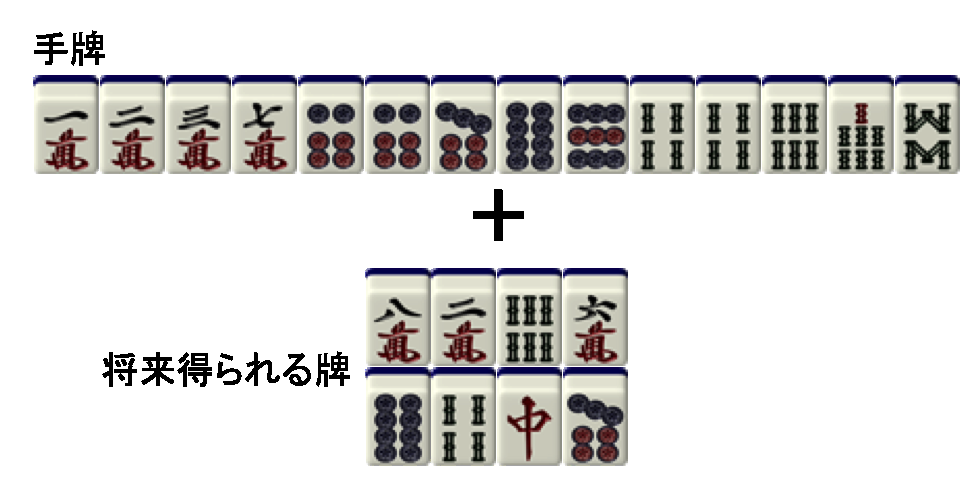
\includegraphics{fig/tehaifuture.eps}
	\end{center}
 	\caption{残り巡目8巡のときの手牌と将来得られる牌を仮定した例}
 	\label{tehaifuture}

	\begin{center}
  		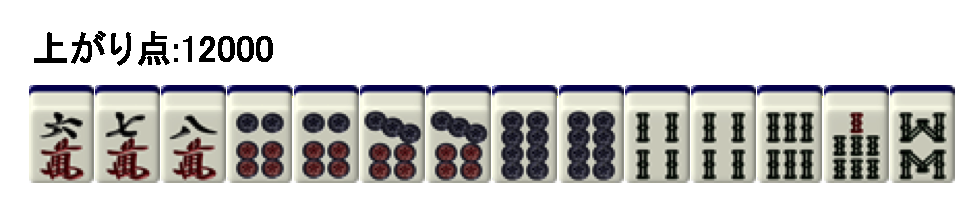
\includegraphics{fig/maxcombination.eps}
	\end{center}
 	\caption{図~\ref{tehaifuture}の牌で上がり点が最大となる組み合わせ}
 	\label{maxcombination}
\end{figure}

\begin{algorithm}[t]
\caption{小松らの手法}
\label{komatu}
	\KwIn{手牌$T$}
	価値を格納する要素数14の配列$V$の各要素を0にする\;
	\For{$i=1$ \KwTo $N$}{
		残り巡目数分の牌をランダムに仮定する\;
		この牌と手牌で上がり点が最大となる組み合わせを求める\;
		\For{$j=1$ \KwTo $14$}{
			\If{$j$番目の牌が組み合わせに含まれない}{
				$V_j \leftarrow V_j +$報酬(上がり点)\;
			}
		}
	}
	$s \leftarrow \argmax_{1 \le j \le 14} V_j$\;
	\Return $T_s$\;
\end{algorithm}

